\documentclass{vgtc}                % final (journal style)
%documentclass[review,journal]{vgtc}         % review (journal style)
%\documentclass[widereview]{vgtc}             % wide-spaced review
%\documentclass[preprint,journal]{vgtc}       % preprint (journal style)

%% Uncomment one of the lines above depending on where your paper is
%% in the conference process. ``review'' and ``widereview'' are for review
%% submission, ``preprint'' is for pre-publication, and the final version
%% doesn't use a specific qualifier.

%% These few lines make a distinction between latex and pdflatex calls and they
%% bring in essential packages for graphics and font handling.
%% Note that due to the \DeclareGraphicsExtensions{} call it is no longer necessary
%% to provide the the path and extension of a graphics file:
%% 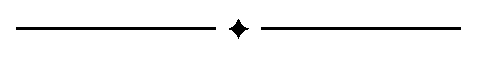
\includegraphics{diamondrule} is completely sufficient.
%%
\ifpdf%                                % if we use pdflatex
  \pdfoutput=1\relax                   % create PDFs from pdfLaTeX
  \pdfcompresslevel=9                  % PDF Compression
  \pdfoptionpdfminorversion=7          % create PDF 1.7
  \ExecuteOptions{pdftex}
  \usepackage{graphicx}                % allow us to embed graphics files
  \DeclareGraphicsExtensions{.pdf,.png,.jpg,.jpeg} % for pdflatex we expect .pdf, .png, or .jpg files
\else%                                 % else we use pure latex
  \ExecuteOptions{dvips}
  \usepackage{graphicx}                % allow us to embed graphics files
  \DeclareGraphicsExtensions{.eps}     % for pure latex we expect eps files
\fi%
\usepackage{caption}
%% it is recomended to use ``\autoref{sec:bla}'' instead of ``Fig.~\ref{sec:bla}''
\graphicspath{{figures/}{pictures/}{images/}{./}} % where to search for the images

\usepackage{microtype}                 % use micro-typography (slightly more compact, better to read)
\PassOptionsToPackage{warn}{textcomp}  % to address font issues with \textrightarrow
\usepackage{textcomp}                  % use better special symbols
\usepackage{mathptmx}                  % use matching math font
\usepackage{times}                     % we use Times as the main font
\renewcommand*\ttdefault{txtt}         % a nicer typewriter font
\usepackage{cite}

%% If you are submitting a paper to a conference for review with a double
%% blind reviewing process, please replace the value ``0'' below with your
%% OnlineID. Otherwise, you may safely leave it at ``0''.
%\onlineid{0}

%% declare the category of your paper, only shown in review mode
\vgtccategory{Research}

%% Paper title.
\title{Visualizing Earthquake Simulation Data}

%% This is how authors are specified in the journal style

%% indicate IEEE Member or Student Member in form indicated below
\author{Zhenge Zhao\thanks{zhengezhao@email.arizona.edu}, Youhao Wei,\thanks{youhaowei@email.arizona.edu} Joshua A. Levine\thanks{josh@email.arizona.edu}, Matthew Berger\thanks{matthewberger@email.arizona.edu}, Danilo Motta\thanks{ddanilomotta@gmail.com}, Carlos Scheidegger\thanks{cscheid@email.arizona.edu}}
%%\affiliation{\scriptsize University of Arizona}


%other entries to be set up for journal
%\shortauthortitle{Firstauthor \MakeLowercase{\textit{et al.}}: Paper Title}

%% Abstract section.
\abstract{
  Computer simulations of the effect of earthquakes on built structures promise to let engineers understand different tradeoffs and designs at an attractively low cost.
  In this scenario, the bottleneck for the expert is one of \emph{data understanding}: how do different building designs respond to different earthquakes?
  What do the building failure modes have in common, and how does this compare to theoretical predictions?
  The way in which a building responds to an earthquake is complex and controlled by different factors.
  In this poster, we present ongoing work in building a system for interactive visualization of earthquake simulation data, in collaboration with civil engineers who have run thousands of simulations, varying the height of the simulated buildings, ground acceleration, and building structure design.
  We describe the challenges in the visualization of such multivariate time series data, and some of our proposed solutions.
} % end of abstract

%% Keywords that describe your work. Will show as 'Index Terms' in journal
%% please capitalize first letter and insert punctuation after last keyword
\keywords{Visualization, Multivariate time series, Earthquake Simulation, NLP, Kernel}

%% ACM Computing Classification System (CCS). 
%% See <http://www.acm.org/class/1998/> for details.
%% The ``\CCScat'' command takes four arguments.

%%\CCScatlist{Visualization, Multivariate time series, Earthquake Simulation, NLP, Kernel}


% Comment below to remove teaser figure.

%%Uncomment below to disable the manuscript note
\renewcommand{\manuscriptnotetxt}{}

%% Copyright space is enabled by default as required by guidelines.
%% It is disabled by the 'review' option or via the following command:
% \nocopyrightspace

\vgtcinsertpkg

%%%%%%%%%%%%%%%%%%%%%%%%%%%%%%%%%%%%%%%%%%%%%%%%%%%%%%%%%%%%%%%%
%%%%%%%%%%%%%%%%%%%%%% START OF THE PAPER %%%%%%%%%%%%%%%%%%%%%%
%%%%%%%%%%%%%%%%%%%%%%%%%%%%%%%%%%%%%%%%%%%%%%%%%%%%%%%%%%%%%%%%%

\begin{document}

%% The ``\maketitle'' command must be the first command after the
%% ``\begin{document}'' command. It prepares and prints the title block.

%% the only exception to this rule is the \firstsection command

\firstsection{Introduction} % or "Motivation"

\label{sec:myintro}
\maketitle

\begin{figure*}
      \centering
      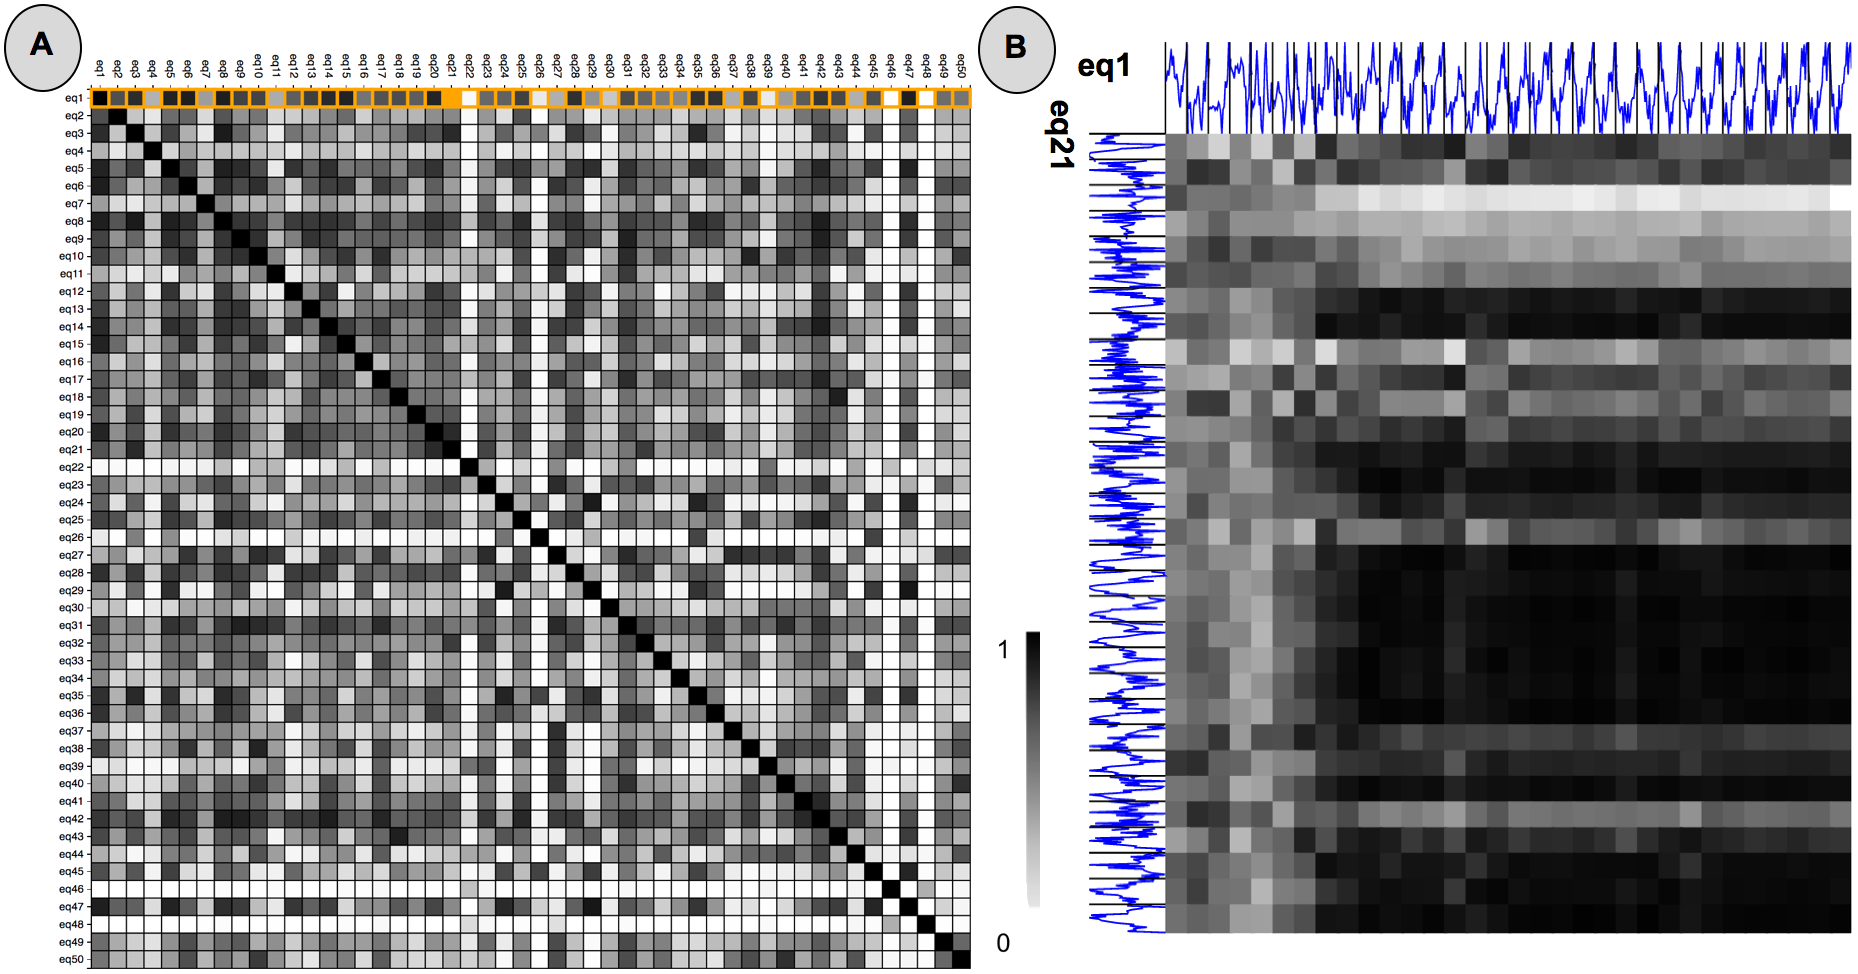
\includegraphics[width=.49\textwidth]{figs/vis1} % first figure itself
      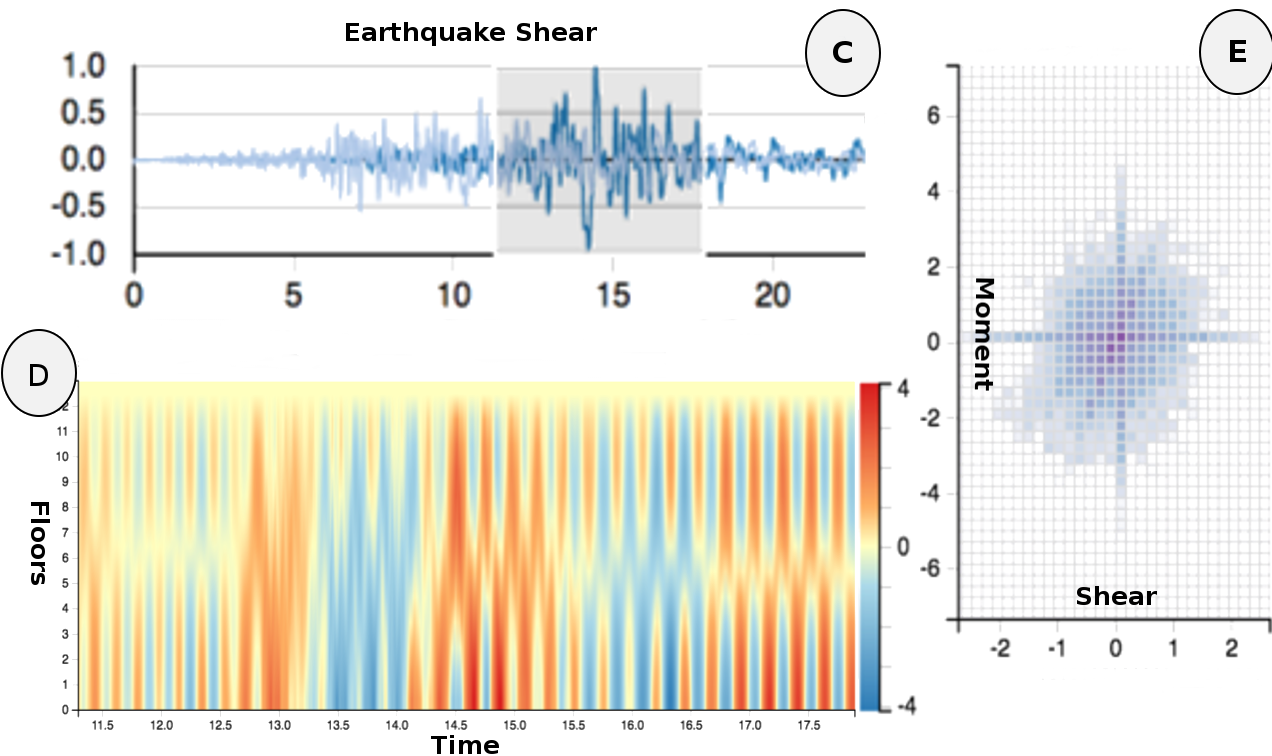
\includegraphics[width=0.37\textwidth]{figs/vis2}
        \caption{Some of the multiple views supporting comparative visualization of earthquake simulations. The response of a building for the entirety of the simulation can be compared to one another, and some earthquakes have more similar responses to others. This gives a comparative overview of all simulations in (A), where a matrix diagram view shows the overall similarities of floor shear across 50 earthquake simulations. In addition, building responses tend to be vibrational and periodic in nature, so segments of an earthquake simulation are compared to one another in (B), where a matrix diagram view demonstrates the similarities between different segments of two earthquake simulations (eq1 and eq21 in view (A)). Analysts can select a portion of the ground acceleration (C) and drill down into a specific earthquake simulation (D), to visualize the response of a single physical variable plotted over time (x coordinate) and building floor (y coordinate). Finally, a 2D histogram can be used to compare two different attributes over the same period of time: how does shear (x coordinate) compare to moment (y coordinate)?\label{fig:teaser}}
\end{figure*}

Through computational simulation, civil engineers can understand how buildings respond to external forces much more efficiently than previously possible.
The simplicity with whcih different scenarios can be simulated and analyzed is attractive, but it is ultimately the source of a new problem: the understanding of the phenomenon is now dependent on the ability to quickly make sense of large amounts of data.

In this poster, we will report on an ongoing collaboration with civil engineers who run a large number of simulations of building responses, and how data analysis and information visualization can highlight interesting patterns in the data.
This problem is especially challenging because of the variety of scales involved. There are multiple earthquakes to be compared to each other; each building's response to an earthquake naturally varies across simulation time, and has different values along different points of the building. There are also periodic phenomena in each simulation, occurring at potentially different periods. Finally, there are multiple physical variables of interest, including shear, moment, and diaphragm forces.

Some of the visualization techniques we using include matrix diagrams and multivariate time series visualizations, as can be seen in Figure~\ref{fig:teaser}. We combine those techniques with classical techniques from signal processing for segmentation, and recent techniques in machine learning for determining similarities between segments of each earthquake simulation.

% Introduction and/or Motivation
%% Analyzing the mechanical structure of different building stories, finding the failing reason when an earthquake attacks a building and investigating the impact of different physical attributes produced by various earthquakes has been a feature of human survival dating back to 230 BC, when ancient Chinese recorded the first earthquake in Puzhou. In efforts to build safer building, understanding earthquake simulation data, for example, the shear stress of each story along the entire time stamps which an earthquake generates when it is shaking a building, is a long-time pursuing for civil engineers. 

%% Nevertheless, currently such tasks can't not be handled and completed perfectly because of the high complexity of the simulation data and the fact that previous work mainly focus on the earthquake itself instead of the simulation data. From visualization perspective, how to visualize such multivariate, multi-scale temporal data remains unclear and potential. In this work, using D3 library~\cite{Bostock:2011:DDD:2068462.2068631},we are trying to design a bunch of visualization views which could help me observe and explore the intricate dataset from different perspectives. Furthermore, we also tried to apply NLP model and kernel methods to these data cubes for comparing them from earthquake level which will be a huge help for the future classification and other machine learning tasks.

%% Besides, the ais of this research is that we also want to compare these earthquake simulation data from different levels. For example, comparing different attributes, what the relation between Shear and Diaphragm Force (two different forces changed during earthquake ) when the earthquake happens. And also what's the behaviour of shear stress among different stories.

% Maybe you want to use a list:

%The rest of the paper isSection~\ref{sec:vis}


%\section{Background}
\label{sec:background}

Collaborative-filtering is a recommendation approach that uses similarity between users and the benefit they have received from items in the past to make recommendations. Three main approaches to collaborative filtering are memory-based, model-based and hybrid methods~\cite{Su:2009:SCF:1592474.1722966} . Memory-based approaches, specifically item-based recommender~\ref{fig:predict}, use an item-user rating matrix to compute pairwise similarities between items. In the contexts of courses, enrollment roster, previous courses students taken and grades course give, is a natural way to reason about course similarity.  

\begin{figure}[h]
 \centering % avoid the use of \begin{center}...\end{center} and use \centering instead (more compact)
 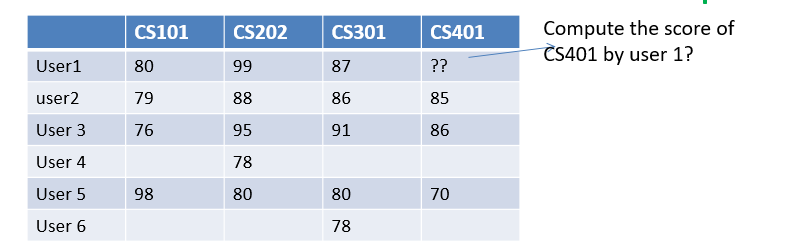
\includegraphics[width=\linewidth]{figs/predict}
 \caption{Typical student course grade table}
 \label{fig:predict}
\end{figure}

However the recommendation approaches are not appropriate for our problems, since they are used for making predictions which means, the approach is designed to fill in the missing values in the matrix. For our case, however, we want to figure out how two courses are correlated with each other. We don’t want to fill the matrix since it will blur the original data. What’ more, for each two courses we are only interested in the users who take both of them. Visualization is an effective and intuitive way to approach our goal.  

There’re many existing similarity measures to compare two entities. Well known metrics include Euclidean similarity, Jaccard(Tanimoto) similarity, Pearson Correlation Coefficient, cosine similarity and Log-likelihood similarity etc. Euclidean similarity measures the distance between courses grading vectors. Jaccard(Tanimoto) similarity is calculated by dividing the intersection of the sets by the union of those sets\cite{sandvig2005aacorn}. Cosine Similarity envision user’s ratings as points in space and measures the cosine of the angle between these lines drawn from origin to each point. The Log-likelihood similarity is a measure of how often items from 2 sets appear together versus how often they appear apart. Pearson Correlation Coefficient is a number between -1, 1. It measures the tendency of the rating vectors, paired one by one, and it’s typically used in early research papers. Its formula is given as $pearson-correlation(u,w) = \frac{cov(R_u,R_w)}{\sigma x \sigma y} $ where $cov$ stands for covariance and $\sigma x$ stands for standard deviation of $x$. We are interested in the strong positive correlation and the positive correlation as illustrated in~\ref{fig:psc}.

For our work, Euclidean similarity is not suitable because courses taken by more students will be added more distances. Jaccard(Tanimoto) similarity and Log-likelihood don’t count grades students get. We choose Pearson Correlation coefficient to indicate the similarity between two courses and based on that, we build our item-based recommender system and provide a way to measure the benefits between two courses.
\begin{figure}[h]
 \centering % avoid the use of \begin{center}...\end{center} and use \centering instead (more compact)
 \includegraphics[width=1.5in]{figs/psc_illustrated}
\caption{Pearson Correlation Illustrated}
 \label{fig:psc}
\end{figure}




\section{Related Work}
\label{sec:related}

Although the problem of understanding how a building behaves during an earthquake has long been studied.
In order to investigate the performance of a building on a shake table, in 2007, engineers built a seven-story building for testing and re-creation of a seismic response of it based on recorded data of a full scale shake table test~\cite{Chourasia:2007:DRS:1247238.1247243}. Here, we are concerned about the relationship between the different physical measurements, as well as with the understanding of how these patterns are similar or different across different earthquakes.

At the same time, visual exploration of multivariate data sets is an integral part of scientific visualization. As in most real world phenomena, there exist multiple factors associated with the complex interactions of different variables. To gain an in-depth understanding of a scientific process, the relationship among the variables needs to be thoroughly investigated. Biswas et al.~\cite{Biswas:2013:AIFEMDS:1077-2626} propose a framework to classify isocontours of variables based on the relationship between them and users can explore the multivariate data sets using their interface. Comparing time series data is another great challenge. Kernel methods, such as Support Vector Machines and Gaussian Processes have become classical data-analysis tools. Vert et al. propose an alignment kernel for time series which is widely used when comparing time series~\cite{DBLP:journals/corr/abs-cs-0610033}.




\section{Research Plan} % or "Research Plan"
\label{sec:vis}

Our ultimate goal is to find a decent way to compare these multi-variate temporal data and design a visualization tool for civil engineers to interactively explore the whole dataset and understand the data. We talk with them about what they need to summarize our tasks as below:
\begin{itemize}
	\item [T1] Overview of clusters of the all the earthquake simulations 
	\item [T2] For a specific earthquake simulation, design a visualization view to explore the multiviate dataset
	\item [T3] For the two views above, build efficient navigation and interaction between them 
\end{itemize} 


\subsection{Data Structure}
\label{sec:data}
\begin{figure}[h]
	\centering % avoid the use of \begin{center}...\end{center} and use \centering instead (more compact)
	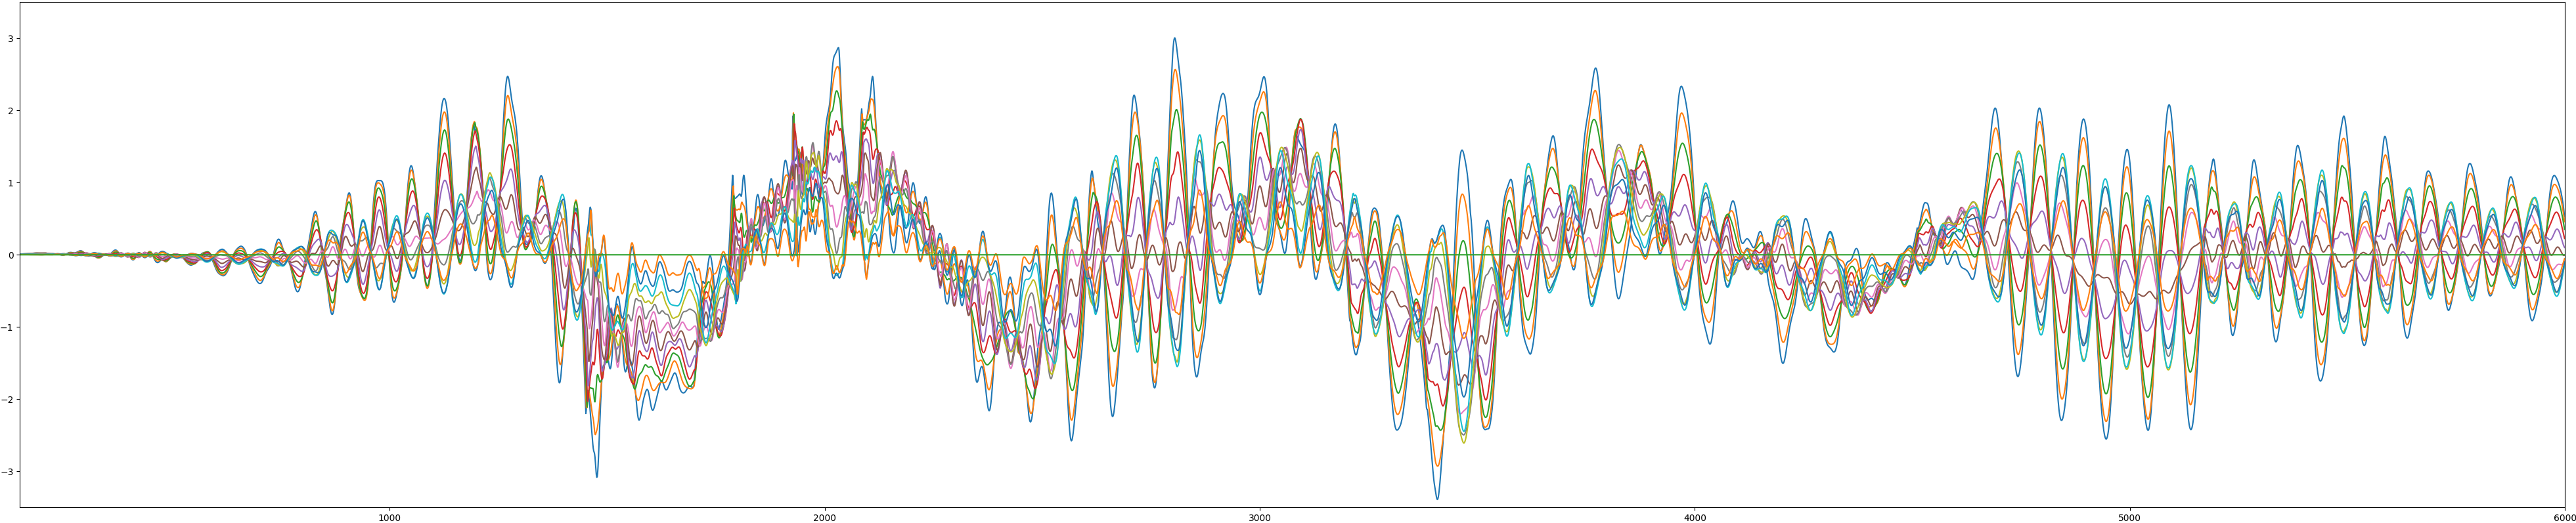
\includegraphics[width=\columnwidth]{figs/eq} 
	\caption{time series for "Shear" attribute of one earthquake simulation}
	\label{fig:data}
\end{figure}

Towards this end, we performed a pilot study using  earthquake simulation data generated by applying 50 different earthquakes to shake a 12-story building. The civil engineers calculated 6 attributes data, Acceleration/PGA, Shear, Diaphragm Force, Moment, Drift Ratio, Interstory Drift Ratio. For example,Shear is the stress component parallel to a given surface, such as a fault plane, that results from forces applied parallel to the surface or from remote forces transmitted through the surrounding rock. For each attribute, there are 13 time series data consponding to 12 stories plus the ground. Then all the data are  normalized and centered. Fig. 3 is one earthquake's Shear simulation time series for 13 stories which indicated by 13 different colors. Fig. 4 is the structure of the whole dataset. Right now, in terms of comparing different simulation data, we have not extended to the cubic including attribute dimension which is the shading part.
\begin{figure}[h]
	\centering % avoid the use of \begin{center}...\end{center} and use \centering instead (more compact)
	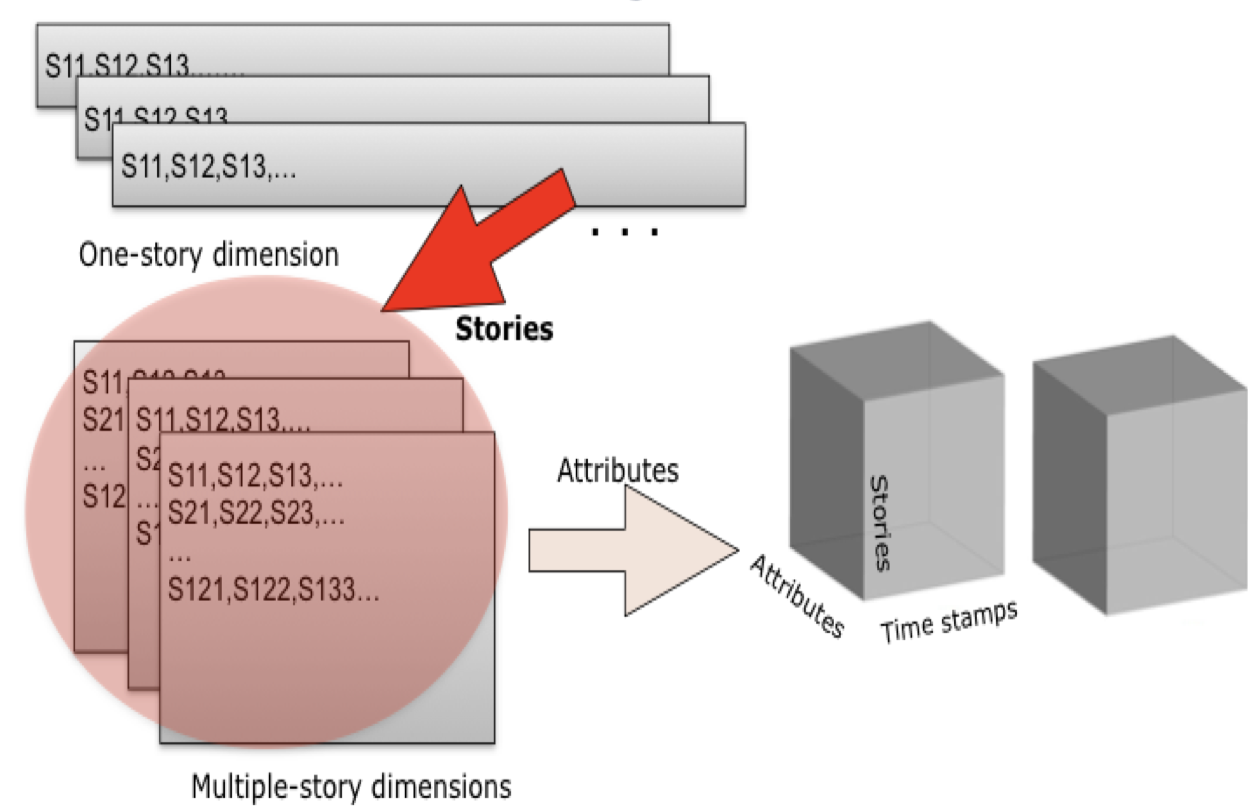
\includegraphics[width=\columnwidth]{figs/structure} 
	\caption{The overall structure of the earthquake simulations, the shading part what we are working on right now}
	\label{fig:data}
\end{figure}


\subsection{Detailed Data View}
\label{sec:context }
This visualization view(Fig. 2) give users a way to explore one cubic database. It includes three parts: two time series plots for accerlation data, A heatmap plot for the time series of the other attributes and a 2D histogram to demonstrate the data value distribute of two selected attribute. The accerlation is the atrribute of the earthquake itself which will be same for all the stories at the same time stamps. We list it individually and these two plots obeying overview + details on demand which allows you to zoom and brush any  time intervals. In the heatmap, you can see the heatmap one attribute of this earthquake simulation data, you can navigate among different attributes and colormaps. The 2D histogram allow you to compare the the selected attribute in part B and any other attribute. Some interactions are built between between differrent parts which allow you to discover rare patterns and models.

\subsection{Overview View}
\label{sec:context }

\subsubsection{NLP Model and Probability Product Kernel}
\label{method}
The other view (Fig. 1) organize the whole dataset under a much more abstract way. Now we want to compare the Shear value among different earthquake data. Based on the fact and observation that earthquakes data has some repeated periods (Fig. 2).  We applied a big-of-words model to cut each earthquake simulation into a set of segments with a fixed period(P), the P is found using cross-correlation within itself. Each segment is a 13XP matrix.After applying the chopping method, each earthquake simulation becomes a set of matrices(motifs). For any two motifs coming from any two earthquakes, we could always calcuate the cosine similarity if we upsample one motif to the same length of the other. Eventually we could calculate the similarity of any two earthquake simulations with the same attribute. In order to capture more features and solving the problem that cross-correlation is not a kernel which may hurt the futher classification. we implicitly map these segments to a Hilbert Space and fit a Gaussian distribution to each earthquake simulation using Kernel PCA.~\cite{conf/icml/KondorJ03} Then we measure the similarity between earthquake simulations as Bhattacharyya’s measure of affinity between such Gaussians.
%TODO: add formula
\subsubsection{Matrix view}
\label{matrixvis}

The Adjacency Matrix view enables users to grasp a global view of one attribute among the all simulation data. We use D3 library which contains the existing adjacency matrix template~\cite{Bostock:2011:DDD:2068462.2068631}. Each grid in the matrix represents the similarity between two simulation data on this attribute.  We build a mouse over in this view, when the users move their mouse on the grid, the column and the row associated with that gird chosen will be highlighted with a bold border which will make it easier to obverse the column and the row. The view also consists a zoomable and navigation feature which can be used to filter the uninterested data based on the demand. Click on one of the grid will give another matrix comparing all the motifs from one earthquake simulation with all the motifs from the other.Theses two views allow users to explore interesting finding. For example, in Fig. 1, the first earthquake is similar to most of the others, the fifteenth, however, is quite different from the others. Clicking any of the label of the earthquake will also allow you navigate to the context view to further study the earthquake simulation you identify.


\
%\begin{figure*}[h]
% \centering 
% 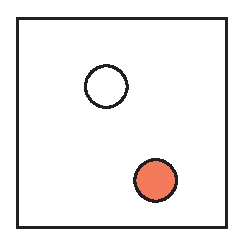
\includegraphics[width=\textwidth]{figs/sample} 
% \caption{Double Column Figure.}
% \label{fig:sample2}
%\end{figure*}



%\section{Evaluation} % or "Research Plan"
\label{sec:vis}

In this section, we show some user studies and the results of your visualization. Since our data comes from a real world university, we can actually know the contents of each course and by consoling computer scientists, we can see if Coursim actually gives us some good perquisites for a chosen course. We also show our evaluation plan here for doing an actual user study.

\subsection{Usage Scenario}
\label{sec:usage}

This case study shows three different usages of this tool. First, when a student comes to his advisor and asked him a question like “what courses do I need to take this semester if I eventually want to take CS482?” The professor doesn’t know how much about CS482, actually the professor is just a Math Doctor which his student takes the CS as a minor. But using our tool, when can find the course CS482 in the adjacency matrix and click the column. Then in the bar chart ( Fig. 8), he can easily figure out that the CS130 and CS343 have the highest benchmarks. Then he moves to the matrix and clicks on the gird of pair CS130 –CS482 and CS343-CS482. The parallel oordinates tell him the most the students are enhanced if they have taken CS130 and CS343. With this knowledge in mind, he can advise the two courses to his students without knowing what actually the two courses are. What's more, another interesting question a student may be wondering is that if he has taken a course, which course he may take next which will be easiler for him to get a high score. For this purpose, he can find the row of that course, and go through the row and find out the red girds. Then he can click on it and see the details in the bar chart and parallel coordinates. The last example is that it can be used to evaluate the setting of  the current prerequisites. We can easily achieve that by finding out the pair of courses and watch its actual ranks in the barchart. Using the bar chart and parallel, a professor can figure out if the current prerequisites is a good. Are there any other hidden prerequisites which have a higher benefit than the current one? Or what’s actual performance looks like for students taking the prerequisites?

After plotting the pictures, we want to find out if the benchmarks work well. We pick up some pair of courses and find out the contents and titles of the university’s websites. The results shown are quite interesting. For example CS 365 and CS489, the benchmark we calculate is 11.2. CS365 is  Model of Computation and CS 489 is a topic course which includes Big Data Infrastructure, Complexity of Computational Problems and Introduction to Machine Learning, which include a lot of model computation.Some other pairs of courses with high benchmarks are also convinced by different domain specialists there are a lot of connections between these pairs. For instance, CS 135 Designing Functional Programs and CS 445: Software Requirements Specification and Analysis, CS 458: Computer Security and Privacy-CS 456 Computer Networks.


\subsection{Evaluation Plan}
\label{sec:plan}

As we stated in the original proposal, an intermediate evaluation test would be comparing documented dependency to the overview drawn by our tool. The overview should be a superset of documented dependency but not close to a universal set. We can worry less about false positives because the prototype doesn't have a high density of highlighted cells.

The above test can be automated relatively easily. We may not even need to get user involved. The ratio of identified documented dependency over all documented dependency should be the prime and only thing to look at in my opinion.

After that, an evaluation of false positives may be carried out. I see two possibilities: first is to contact the academical advisor from our dataset's university to confirm the possible dependency revealed by our tool; second is to find a local academical advisor who is willing to share her data and apply our tool to it. In fact, doing both would be more convincing.

Eventually, a user study should be done. We should have an academical advisor's feedback and improved the tool at this moment. We then ask the academical advisor to use this tool with students seeking advice, when they choose their courses. We need to be careful about the user groups here. Do we want to work with the same academical advisor all the time? Do we care about gender balance, student year(freshman, senior) balance?

I think we should share this tool with a handful of academical advisors, to avoid the tool being too personalized. When their feedback conflicts, we record their argument first and ask them if they are willing  to discuss further. We end up either solving the issue or having one implementation but understanding the alternatives. 

For a balanced student group, the question boils down to who's going to actually use this tool. If the tool is going to be used sololy with both student and academical advisor in presence, then we should accept whoever comes to the office and don't worry about balance at all. If the tool is going to be offered in the school system open to all students, we should invite students to evaluate it online in addition to academical office deployment. I'm more inclined to the first approach simply because it is easier to come true.

Existing tools should be considered in doing all these evaluations. A survey should be taken, asking users to rate all three views on a Likert scheme, with an optional text box of why they like or hate any part. Depending on the skewness, we maybe need to throw away the top 5\% high and low gradings. The text feedback should be synthesized to explain the gradings of each view and discussed possible improvement.


%\section{Discussion}
\label{sec:discussion}

The project is successful overall. We learned valuable lessons throughout. They are about both general research and visualization research.
\begin{itemize}
\item Knowing what's out there in the field is important. Researchers at entry level often start out experimenting their own thoughts without studying literatures. Reference is more than citation. Readers will not be convinced unless we can relate other people's work to ours and explain why, how, and what we are doing differently.
\item During this project, we find it really helpful to summarize the problems of published papers. These problems serve as good reminders of common pitfalls even for experienced researchers and reviewers. We also think going back to the first slides at the beginning of semester to be useful. It helps keep the project going in a regular track.
\item For the coding part, d3 is a quite different language from C-style ones. We started out skimming preliminary tutorials and moved on to modify the gallery codes. This approach turned out to be inefficient and painful. I personally misunderstood chaining methods until mid term. If one happens to be familiar with C-style languages like me, d3 is likely to deserve more time to acquire than you anticipate.
\item Time management is crucial. It's dangerous to wait till last minute. We usually set for ourselves a dummy deadline, one or two days prior to the real deadline. We thus apply major fixes early and have enough time for minor fixes in a relaxed mood, which actually improves the quality of those minor fixes.
\end{itemize}



\paragraph*{Ongoing work}
\label{sec:conclusion}

Now let's review our tasks listed in Section 3. For task 1, we applied a NLP model and different kernel methods to summary the simulations as much as we can to get a overview quantitatively. For task 2, we build a context visualization to illustrate the details of the specific simulation. The design principle of this view is to remain the ground truth as much as possible. For task3, we follow the focus and context design, which allows user to spot the earthquake simulation they are interested and explore it in the context view. The prototype looks promising for now, since it provides a way to explore the whole earthquake dataset. In the meanwhile, there are  a lot of points for us to complete.

Even with the matrix diagram visualizations, the screen becomes cluttered as the number of simulation gets larger. In the future, when we get thousands of simulations, the matrix diagram will not scale. It is also worth considering if it's possible to cluster earthquakes hierarchically to maintain visual scalability. The way we choose periods for segmentation is also clearly inappropriate; we are currently investigating how to enable our machine learning methods with multiple overlapping motifs ([T3]).
Finally, even though we have worked with domain experts in developing these tools, a thorough validation of the designs, for example,   efficient navigation and interaction between different views, remains to be done.


%\bibliographystyle{abbrv}
\bibliographystyle{abbrv-doi-hyperref}
%%use following if all content of bibtex file should be shown
%\nocite{*}
\bibliography{report}
\end{document}

